\section{Recap}

\begin{frame}[fragile]\frametitle{R syntax - \texttt{glm()} vs \texttt{lm()}}
  \begin{itemize}
  \item the \texttt{glm()} function needs
    \begin{itemize}
    \item a model formula (like \texttt{lm})
    \item the specification of error distribution (\texttt{family=})
    \end{itemize}
  \end{itemize}
\begin{exampleblock}{Input/Output}\small
\begin{verbatim}
> m1 <- lm(bweight ~ hyp, data=births)
> m2 <- glm(bweight ~ hyp, family=gaussian, data=births)
\end{verbatim}
\end{exampleblock}
\end{frame}

\begin{frame}\frametitle{\texttt{glm()} for logistic regression}
  \begin{itemize}
    \item every error family has a canonical link
    \item we have seen binomial error family with its canonical logit link
    \item common choices for link functions used with binomial errors
      \begin{itemize}
      \item logit: $\eta = \log(p/(1-p))$
      \item probit: $\eta = \Phi^{-1}(p)$ 
      \item log-log: $\log(-\log(1-p))$
      \end{itemize}
  \end{itemize}
\end{frame}


\begin{frame}\frametitle{Odds}
  \begin{itemize}
    \item logistic regression is more understandable if you look at the coefficients in terms of odds where
    \item $\Omega(A) = \frac{P(A)}{1-P(A)}$
    \item so what are the corresponding odds for a probability of
      \begin{itemize}
      \item $p = 1$
      \item $p = 0.99$
      \item $p = 0.5$
      \item $p = 0.1$
      \item $p = 0.01$
      \item $p = 0$        
      \end{itemize}
  \end{itemize}
\end{frame}


\begin{frame}\frametitle{Odds}
\begin{columns}
  \begin{column}{0.4\textwidth}
    $$p = 1$$
    $$p = 0.99$$
    $$p = 0.5$$
    $$p = 0.1$$
    $$p = 0.01$$
    $$p = 0$$    
  \end{column}
  \begin{column}{0.4\textwidth}
    $$\omega = \infty$$
    $$\omega = 99$$
    $$\omega = 1$$
    $$\omega = 0.\bar{1}$$
    $$\omega = 0.\overline{01}$$
    $$\omega = 0$$
  \end{column}
\end{columns}
\end{frame}


\begin{frame}[fragile]\frametitle{Remember the Data}
\footnotesize
\begin{exampleblock}{Input/Output}
\begin{semiverbatim}
  > str(births)
  'data.frame':	500 obs. of  8 variables:
 $ id     : num  100 101 102 103 104 105 106 107 108 109 ...
 $ preterm: Factor w/ 2 levels "preterm","normal": 2 2 2 2 2 2 2 NA 2 2 ...
 $ gestwks: num  39.8 39 38.1 39.5 39.5 ...
 $ hyp    : Factor w/ 2 levels "normal","hyper": 1 1 1 1 2 1 2 1 1 1 ...
 $ matage : num  33 32 33 38 40 29 32 40 41 39 ...
 $ bweight: num  3576 3784 2796 3226 3138 ...
 $ lowbw  : Factor w/ 2 levels "normal","low": 1 1 1 1 1 1 1 1 1 1 ...
 $ sex    : Factor w/ 2 levels "M","F": 2 2 2 2 2 2 1 1 2 2 ...
\end{semiverbatim}
\end{exampleblock}
Data from: Michael Hills and Bianca De Stavola (2002). A Short Introduction
     to Stata 8 for Biostatistics, Timberlake Consultants Ltd URL:
     http://www.timberlake.co.uk
\end{frame}

\begin{frame}[fragile]\frametitle{Exercises}
Remember: We used hypertension of the mom to explain variation in the birth weight (in terms of low birth weight or not of course) of the kid. Without looking in the material of the last session, try to redo the model. Here are some hints:
\begin{itemize}
\item of course you need the \texttt{glm()} function
\item you need to specify the formula which has to have the general form $y \sim x$
\item additional you need to specify the data and the error family (in the case \texttt{binomial})
\item use the \texttt{summary()} function on the model
\item use \texttt{Effect()} or \texttt{allEffects()} commands on the model
\item how to interpret the results? Is the effect of hypertension statistically significant?
\end{itemize}
\end{frame}


\begin{frame}[fragile]\frametitle{Exercise - Solution}\footnotesize
\begin{exampleblock}{Input/Output}\scriptsize
\begin{verbatim}
> m <- glm(lowbw ~ hyp, family=binomial, data=births)
> summary(m)
Call:
glm(formula = lowbw ~ hyp, family = binomial, data = births)

Deviance Residuals: 
    Min       1Q   Median       3Q      Max  
-0.8067  -0.4430  -0.4430  -0.4430   2.1773  

Coefficients:
            Estimate Std. Error z value Pr(>|z|)    
(Intercept)  -2.2721     0.1661 -13.682  < 2e-16 ***
hyphyper      1.3166     0.3111   4.232 2.32e-05 ***
---

(Dispersion parameter for binomial family taken to be 1)

    Null deviance: 366.92  on 499  degrees of freedom
Residual deviance: 350.84  on 498  degrees of freedom
AIC: 354.84

\end{verbatim}
\end{exampleblock}
\end{frame}



\begin{frame}[fragile]\frametitle{Exercise - Solution}\footnotesize
\begin{exampleblock}{Input/Output}\small
\begin{verbatim}
> require(effects)
Lade nötiges Paket: effects
> allEffects(m.hyp)
 model: lowbw ~ hyp

 hyp effect
hyp
    normal      hyper 
0.09345794 0.27777778 
> plot(allEffects(m.hyp))
\end{verbatim}
\end{exampleblock}
\end{frame}



\begin{frame}[fragile]\frametitle{Exercise - Solution}\footnotesize
  \begin{center}
    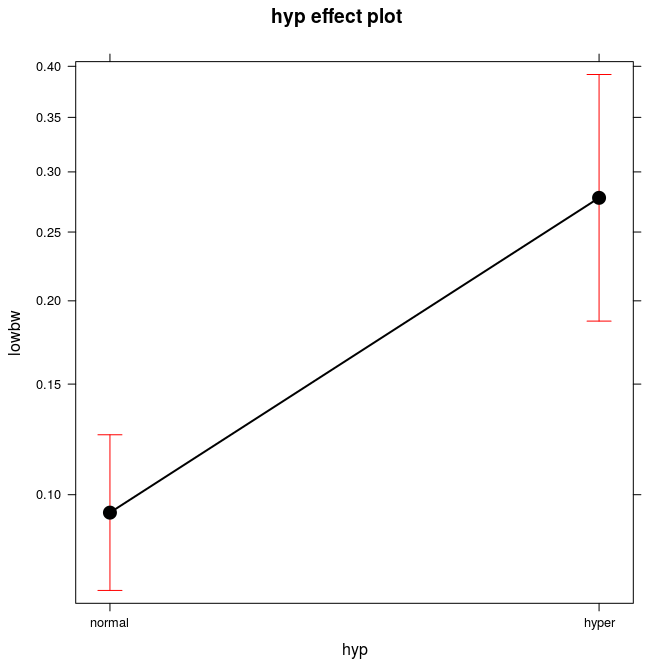
\includegraphics[width = 8cm]{hypeffect.png}
  \end{center}
\end{frame}

\begin{frame}[fragile]\frametitle{Exercise - Solution}\footnotesize
\begin{exampleblock}{Input/Output}\scriptsize
\begin{verbatim}
> res <- allEffects(m.hyp, se = T)
> summary(res)
 model: lowbw ~ hyp

 hyp effect
hyp
    normal      hyper 
0.09345794 0.27777778 

 Lower 95 Percent Confidence Limits
hyp
    normal      hyper 
0.06929267 0.18675845 

 Upper 95 Percent Confidence Limits
hyp
   normal     hyper 
0.1249195 0.3917861 
\end{verbatim}
\end{exampleblock}
\end{frame}

\begin{frame}[fragile]\frametitle{Exercises}
  What is the relationship between the coefficients of the model (from the model summary) and the effects?
\end{frame}


\begin{frame}[fragile]\frametitle{Exercises - Solutions}
  What is the relationship between the coefficients of the model (from the model summary) and the effects?
  \begin{itemize}
  \item we have to use the inverse link function on the coefficients to transform the coefficients on the logit scale to more interpretable probabilities
  \end{itemize}
  \begin{exampleblock}{Input/Output}
\begin{verbatim}
> invlogit(coef(m.hyp)[1])
(Intercept) 
 0.09345794 
> invlogit(coef(m.hyp)[1] + coef(m.hyp)[2])
(Intercept) 
  0.2777778 
\end{verbatim}
  \end{exampleblock}
\end{frame}


\section{Binomial/Logistic Regression}

\begin{frame}[fragile]\frametitle{Simple Logistic Regression}
\begin{itemize}
\item now we model the probability of low birth weight dependent on gestational age (numeric variable)
\item so the model in R is 
  \begin{exampleblock}{Input}\footnotesize
\begin{verbatim}
> m.wks <- glm(lowbw ~ gestwks, family=binomial, data=births)
\end{verbatim}
  \end{exampleblock}\normalsize
\item and as math formula
$$ \log\left(\frac{\mbox{Pr(lowbw)}}{1-\mbox{Pr(lowbw)}}\right) = \beta_0 + \beta_1 \cdot \mbox{gestwks} + \epsilon$$
\end{itemize}
\end{frame}


\begin{frame}[fragile]\frametitle{Simple Logistic Regression}
\begin{itemize}
\item where the output look similar to the output above
  \begin{exampleblock}{Input/Output}\scriptsize
\begin{verbatim}
> summary(m.wks)

Call:
glm(formula = lowbw ~ gestwks, family = binomial, data = births)

Deviance Residuals: 
    Min       1Q   Median       3Q      Max  
-2.0873  -0.3623  -0.2223  -0.1369   2.9753  

Coefficients:
            Estimate Std. Error z value Pr(>|z|)    
(Intercept)  31.8477     4.0574   7.849 4.18e-15 ***
gestwks      -0.8965     0.1084  -8.272  < 2e-16 ***
---
Signif. codes:  0 ‘***’ 0.001 ‘**’ 0.01 ‘*’ 0.05 ‘.’ 0.1 ‘ ’ 1

(Dispersion parameter for binomial family taken to be 1)

    Null deviance: 360.38  on 489  degrees of freedom
Residual deviance: 205.75  on 488  degrees of freedom
  (10 observations deleted due to missingness)
AIC: 209.75

Number of Fisher Scoring iterations: 6
\end{verbatim}
  \end{exampleblock}
\end{itemize}
\end{frame}


\begin{frame}[fragile]\frametitle{Understanding the Coefficients}
\begin{itemize}
\item this relationship is described by $$\mbox{Pr(lowbw)}=\mbox{logit}^{-1}(31.8477 + -0.8965 \cdot \mbox{gestwks}) $$
\item the intercept
  \begin{exampleblock}{Input/Output}
\begin{verbatim}
> invlogit(coef(m.wks)[1])
(Intercept) 
  1
\end{verbatim}
  \end{exampleblock}
is interpretable as the probability for a low birth weight at a hypothetical gestational age of 0 (which makes no sense because it lies outside the range of gestational ages in our data and is nonsense anyway)
\item the parameter for \texttt{gestwks} describes how fast the probability decreases with increasing gestational age
\end{itemize}
\end{frame}

\begin{frame}[fragile]\frametitle{Understanding the Coefficients}
$$\mbox{Pr(lowbw)}=\mbox{logit}^{-1}(31.8477 + -0.8965 \cdot \mbox{gestwks}) $$
\begin{itemize}
\item the coefficient for \texttt{gestwks} is best interpretable if we use it as argument to the exponential function
  \begin{exampleblock}{Input/Output}
\begin{verbatim}
> exp(coef(m.wks)[2])
  gestwks 
0.4080114 
\end{verbatim}
  \end{exampleblock}
this way it is interpretable as odds ratio for low birth weight for a difference of 1 week of gestational age (because we are measuring gestational in weeks as unit)
\end{itemize}
\end{frame}


\begin{frame}[fragile]\frametitle{Exercise}
  \begin{enumerate}
  \item here is a example for the \texttt{Effects()} command for regression
    \begin{exampleblock}{Input/Output}\scriptsize
\begin{verbatim}
> Effect("gestwks",m.wks)

 gestwks effect
gestwks
        25         30         35         40 
0.99992022 0.99299324 0.61574996 0.01779725 
> Effect("gestwks",m.wks,xlevels = list(gestwks = c(20,30,40)))

 gestwks effect
gestwks
        20         30         40 
0.99999910 0.99299324 0.01779725   
\end{verbatim}
    \end{exampleblock}\normalsize
\item use the command to gain the estimated probability of low birth weight for a gestational age of 27 and 36 weeks
  \end{enumerate}
\end{frame}


\begin{frame}[fragile]\frametitle{\texttt{ggplot()} and \texttt{glm()}}
  \begin{itemize}
  \item ggplot2 knows also glms
  \item unfortunately the y-variable needs to be coded in 0s and 1s, but we can do this on the fly with \texttt{as.numeric()}
  \end{itemize}
  \begin{exampleblock}{Input}\scriptsize
\begin{verbatim}
> require(ggplot2)
> ggplot(births,aes(x = gestwks, y = as.numeric(lowbw)-1)) +
+     geom_smooth(method = "glm", family = "binomial",se = F,size = 2) +
+     geom_point(shape="|")  ## adds actual values  
\end{verbatim}
  \end{exampleblock}
\end{frame}


\begin{frame}\frametitle{\texttt{ggplot()} and \texttt{glm()}}
  \begin{center}
    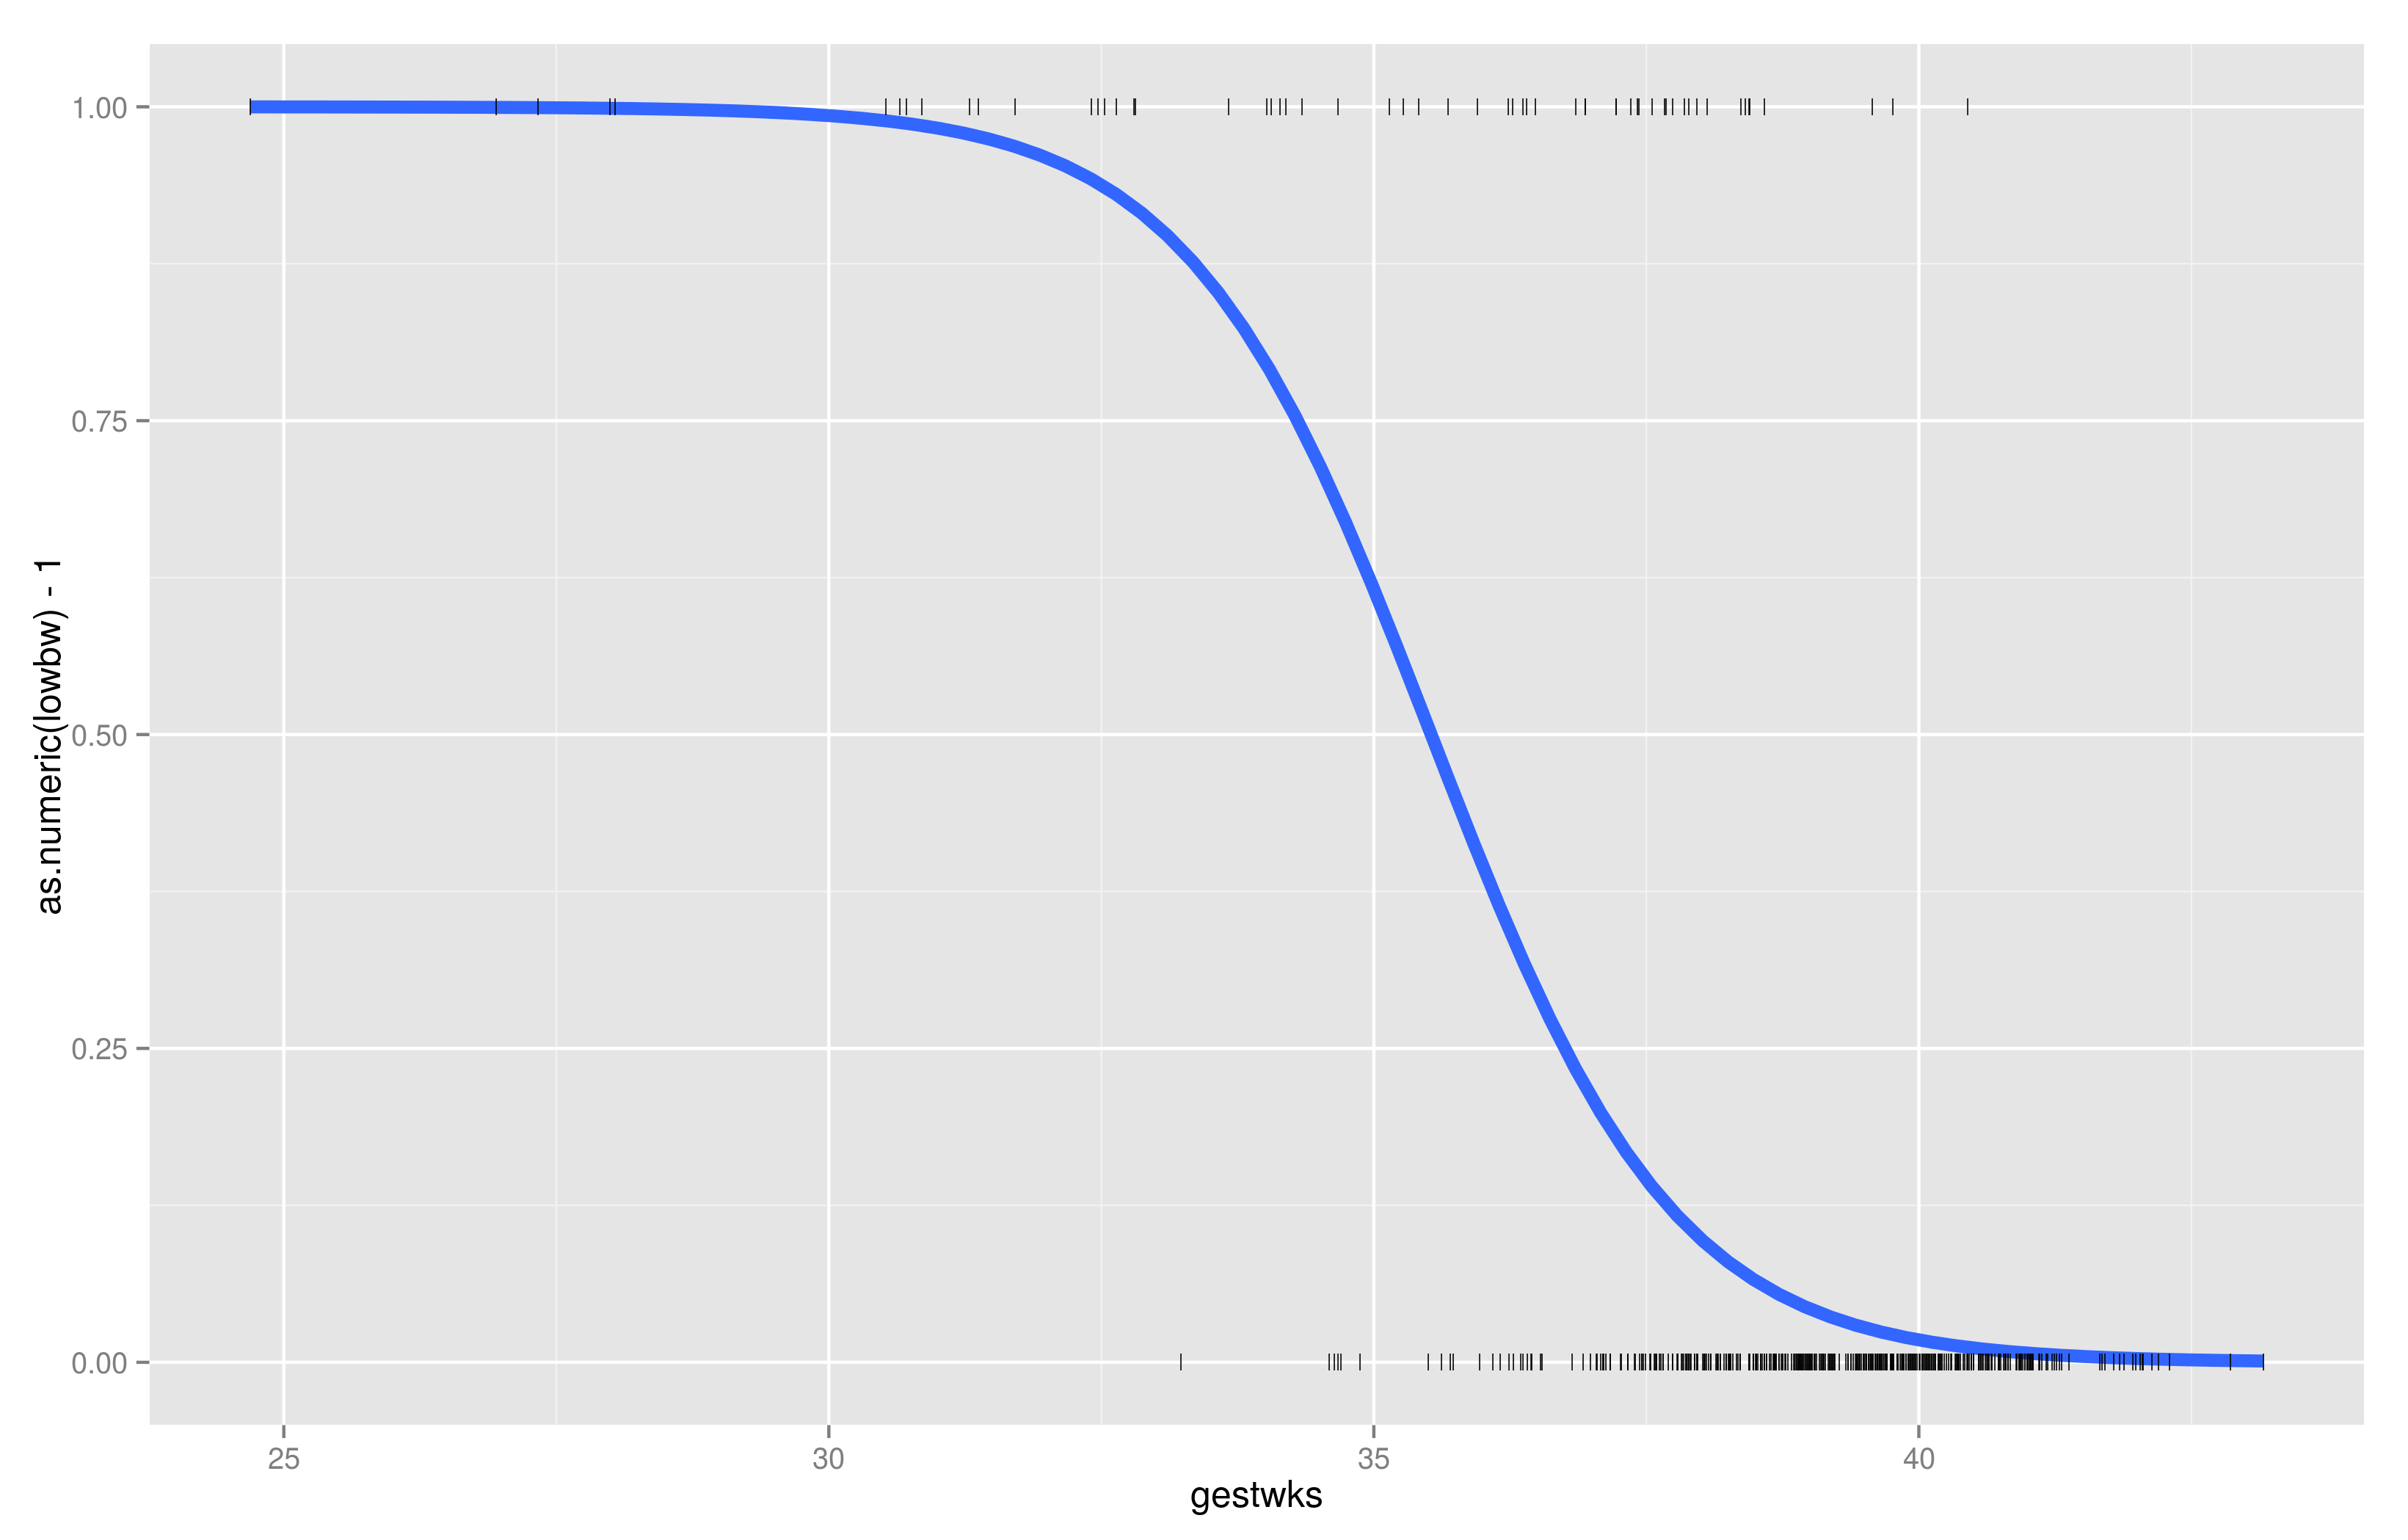
\includegraphics[width=11cm]{glmggplot.png}
  \end{center}
\end{frame}


\begin{frame}[fragile]\frametitle{Exercise}
Take the code producing the graph
  \begin{enumerate}
  \item try to change the axis titles (\texttt{xlab()} and \texttt{ylab()})
  \item add a title (\texttt{ggtitle()})
  \item change the colour of the function to black, set se = T
  \item change the colour of the points to red for the low birth weight and green for the one with normal birth weight
  \item change the position of the legend; place it somewhere near the upper right corner inside the plotting area (\texttt{legend.position})
  \end{enumerate}
\end{frame}

\section{The famous O-Ring example}

\begin{frame}[fragile]\frametitle{The Challenger Disaster Example}
In January 1986, the space shuttle Challenger exploded shortly after launch. An
investigation was launched into the cause of the crash and attention focused on the rubber
O-ring seals in the rocket boosters. At lower temperatures, rubber becomes more brittle
and is a less effective sealant. At the time of the launch, the temperature was 31\degree F. Could
the failure of the O-rings have been predicted? In the 23 previous shuttle missions for
which data exists, some evidence of damage due to blow by and erosion was recorded on
some O-rings. Each shuttle had two boosters, each with three O-rings. For each mission,
we know the number of O-rings out of six showing some damage and the launch
temperature.(faraway)

\url{http://www.history.com/topics/challenger-disaster/videos/engineering-disasters---challenger}

\end{frame}

\begin{frame}[fragile]\frametitle{The Challenger Disaster Example}
\begin{itemize}
\item the data are given in the data frame \texttt{orings} in the \texttt{faraway} package
\item after loading we have a look at the first six lines
  \begin{exampleblock}{Input/Output}\small
\begin{verbatim}
> library(faraway)
> data(orings)
> head(orings)
  temp damage
1   53      5
2   57      1
3   58      1
4   63      1
5   66      0
6   67      0
\end{verbatim}
  \end{exampleblock}

\item we see that every shuttle mission has its own row (but not every O-ring)
\end{itemize}
\end{frame}

\begin{frame}[fragile]\frametitle{The Challenger Disaster Example}
\begin{itemize}
\item that is not a problem: one way of defining a binary response variable in a glm is to form a two-column matrix with the first
column representing the number of “successes” y and the second column the number of “failures” n–y.
\begin{exampleblock}{Input/Output}\small
\begin{verbatim}
> m.oring <- glm(cbind(damage,6-damage) ~ temp,
+                      family=binomial, orings)
\end{verbatim}
\end{exampleblock}

\normalsize
\end{itemize}
\end{frame}

\begin{frame}[fragile]\frametitle{The Challenger Disaster Example}
\begin{itemize}
\item the output looks familiar:
  \begin{exampleblock}{Input/Output}\scriptsize
\begin{verbatim}
> summary(m.oring)
Call:
glm(formula = cbind(damage, 6 - damage) ~ temp, 
     family = binomial, data = orings)
Deviance Residuals: 
    Min       1Q   Median       3Q      Max  
-0.9529  -0.7345  -0.4393  -0.2079   1.9565  
Coefficients:
            Estimate Std. Error z value Pr(>|z|)    
(Intercept) 11.66299    3.29626   3.538 0.000403 ***
temp        -0.21623    0.05318  -4.066 4.78e-05 ***
(Dispersion parameter for binomial family taken to be 1)
    Null deviance: 38.898  on 22  degrees of freedom
Residual deviance: 16.912  on 21  degrees of freedom
AIC: 33.675
\end{verbatim}
  \end{exampleblock}
\item remember, the response is a probability. Therefore our model describes the probability of a damaged O-ring depending on the temperature
\end{itemize}
\end{frame}


\begin{frame}[fragile]\frametitle{Understanding the Coefficients}
\begin{itemize}
\item this relationship is described by $$\mbox{Pr(damage)}=\mbox{logit}^{-1}(11.66299 + -0.21623 \cdot \mbox{temp}) $$
  \begin{exampleblock}{Input/Output}
\begin{verbatim}
> invlogit(coef(m.oring)[1])
(Intercept) 
  0.9999914 
\end{verbatim}
  \end{exampleblock}
\item the intercept is interpretable as the probability for a damaged O-ring at a temperature of 0\degree F
\end{itemize}
\end{frame}

\begin{frame}[fragile]\frametitle{Understanding the Coefficients}
\begin{itemize}
\item the parameter for temperature describes how fast the probability decreases with increasing temperature and it is again best interpretable as odds ratio 
\end{itemize}
\begin{exampleblock}{Input/Output}
\begin{verbatim}
> exp(coef(m.oring)[2])
     temp 
0.8055471 
\end{verbatim}
\end{exampleblock}
\end{frame}


\begin{frame}[fragile]\frametitle{Understanding the Coefficients}\footnotesize
\begin{center}
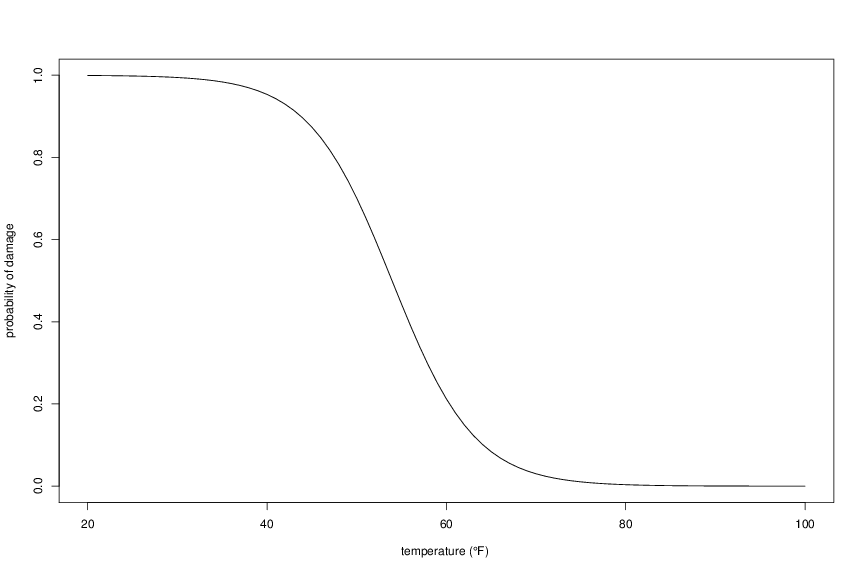
\includegraphics[width=11.5cm]{challenger.png}
\end{center}
\end{frame}

\begin{frame}[fragile]\frametitle{Understanding the Coefficients}
and the same plot made with ggplot (incl. adding a table)
\begin{center}
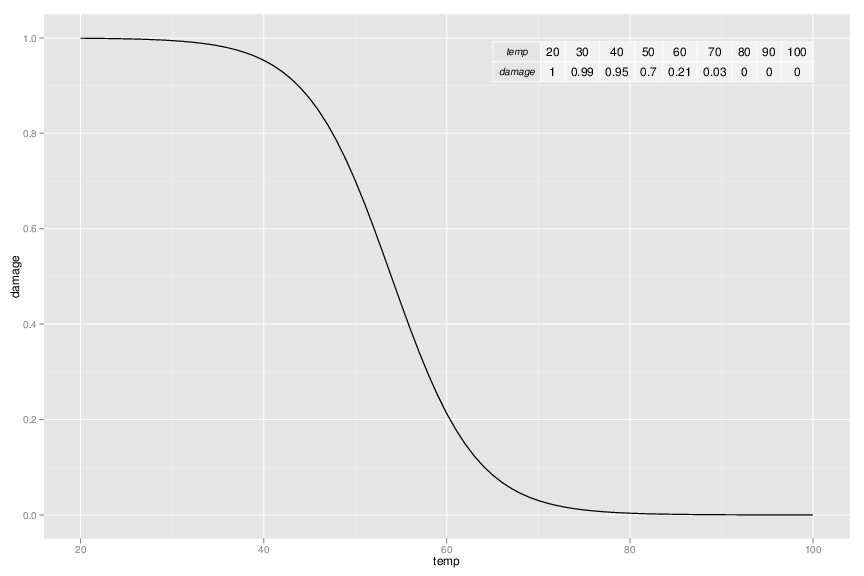
\includegraphics[width=11.5cm]{challenger2.png}
\end{center}
\end{frame}


\section[Binomial Ancova]{Ancova with a Binary Response Variable }

\begin{frame}[fragile]\frametitle{Parasite Infection Example}
\begin{itemize}
\item the binary response variable is parasite infection (infected or not) 
\item the explanatory variables are weight and age (continuous) 
\item and sex (categorical)
\item we want to investigate if there is a different effect of age for each of the sexes on the outcome variable
\end{itemize}
\begin{exampleblock}{Input/Output}\footnotesize
\begin{verbatim}
> load("infection.rdata")
> summary(infection)
         infected        age             sex     
 infected    :338   Min.   :  2.00   female:243  
 not infected:162   1st Qu.: 46.00   male  :257  
                    Median : 84.50               
                    Mean   : 93.69               
                    3rd Qu.:139.25               
                    Max.   :200.00               
\end{verbatim}
\end{exampleblock}

\end{frame}


\begin{frame}[fragile]\frametitle{Parasite Infection Example}\footnotesize
  \begin{exampleblock}{Input/Output}\scriptsize
\begin{verbatim}
> m.inf <- glm(infected~age*sex,family=binomial,
+                               data=infection)
> summary(m.inf)
Call:
glm(formula = infected ~ age * sex, family = binomial, 
                                     data = infection)
Deviance Residuals: 
    Min       1Q   Median       3Q      Max  
-2.0411  -0.7307  -0.4363   0.6632   2.3215  
Coefficients:
             Estimate Std. Error z value Pr(>|z|)    
(Intercept) -3.000513   0.413639  -7.254 4.05e-13 ***
age          0.015657   0.003176   4.929 8.25e-07 ***
sex          0.116664   0.553956   0.211   0.8332    
age:sex      0.011050   0.004612   2.396   0.0166 *  

(Dispersion parameter for binomial family taken to be 1)
    Null deviance: 629.85  on 499  degrees of freedom
Residual deviance: 477.61  on 496  degrees of freedom
AIC: 485.61
\end{verbatim}
  \end{exampleblock}

\end{frame}

\begin{frame}[fragile]\frametitle{Parasite Infection Example}
\begin{itemize}
\item so for male at a age of 0 there is a probability of
    \begin{exampleblock}{Input/Output}
\begin{verbatim}
> invlogit(coef(m.inf)[1])
(Intercept) 
 0.04740269 
\end{verbatim}
    \end{exampleblock}
  \item for females the probability at age 0 is
    \begin{exampleblock}{Input/Output}
\begin{verbatim}
> invlogit(coef(m.inf)[1]+coef(m.inf)[3])
(Intercept) 
 0.05295775 
\end{verbatim}
  \end{exampleblock}
\end{itemize}
\end{frame}


\begin{frame}[fragile]\frametitle{Compare Slopes}
\begin{itemize}
\item so what about the slope?
\item for males the underlying model is the following
$$\mbox{Pr(infection)}=\mbox{logit}^{-1}(-3.000513 + 0.015657 \cdot \mbox{age}) $$
\item for females the slope is almost twice as high
  $$\mbox{Pr(infection)}=\mbox{logit}^{-1}(-2.883849 + 0.02670685  \cdot \mbox{age}) $$
\end{itemize}
\end{frame}


\begin{frame}[fragile]\frametitle{Compare Slopes}
\begin{itemize}
\item looking at the odds ratios (which seem to be rather small)
\item for males and females:
  \begin{exampleblock}{Input/Output}\small
\begin{verbatim}
> exp(coef(m.inf)[2]) ## males
    age 
1.01578 
> exp(coef(m.inf)[2] + coef(m.inf)[4]) ## females
     age  
1.027067 
\end{verbatim}
  \end{exampleblock}
\item these are the odds ratios for +1 time unit
\end{itemize}
\end{frame}

\begin{frame}[fragile]\frametitle{Compare Slopes}
  \begin{itemize}
  \item if time unit is days you get the odds ratio for +1 month   by
  \begin{exampleblock}{Input/Output}\small
\begin{verbatim}
> exp(30 * coef(m.inf)[2])
     age 
1.599512 
> exp(30 * (coef(m.inf)[2] + coef(m.inf)[4]))
     age 
2.228225 
\end{verbatim}
  \end{exampleblock}
\item so keep in mind the scale you are measuring on
\end{itemize}
\end{frame}

  \begin{frame}[fragile]\frametitle{Compare Slopes}
\begin{itemize}
\item we can also compare them by looking at the age where the probability to be infected is 50\%
\item this is the case when $$-3.000513 + 0.015657 \cdot \mbox{age}=0$$  respectively $$-2.883849 + 0.02670685  \cdot \mbox{age}=0$$ you can do it by hand or use R
\end{itemize}
\end{frame}

\begin{frame}[fragile]\frametitle{Compare Slopes}
\begin{itemize}
\item \texttt{solve()} solves systems of linear equations in the form A*x=b, where A is the matrix of coefficients and b are the (negative) intercepts, here we have the special case with just one equation
  \begin{exampleblock}{Input/Output}\small
\begin{verbatim}
> ## male
> solve(0.015657,3.000513)
[1] 191.6404
> ## female
> solve(0.02670685,2.883849)
[1] 107.9816
\end{verbatim}
  \end{exampleblock}

\end{itemize}
\end{frame}

\begin{frame}[fragile]\frametitle{Compare Effects}
\begin{itemize}
\item you can also use the \texttt{allEffects()} function (part of the \texttt{effects} package), which give you the probabilities for being infected on several ages for both sexes
  \begin{exampleblock}{Input/Output}\scriptsize
\begin{verbatim}
> allEffects(m.inf)
 model: infected ~ age * sex

 age*sex effect
     sex
age            0          1
  2   0.04883687 0.05570148
  24  0.06756215 0.09596497
  46  0.09276694 0.16038932
  68  0.12610300 0.25582483
  90  0.16918450 0.38219715
  112 0.22322468 0.52680374
  134 0.28853152 0.66704908
  156 0.36399154 0.78286130
  178 0.44679328 0.86645480
  200 0.53265591 0.92110968
\end{verbatim}
  \end{exampleblock}

\end{itemize}
\end{frame}


\begin{frame}[fragile]\frametitle{Compare Effects}
\begin{itemize}
\item choose values of age
  \begin{exampleblock}{Input/Output}\footnotesize
\begin{verbatim}
> allEffects(m.inf,
+            xlevels = list(age = seq(0,200,by = 50)))
 model: infected ~ age * sex

 age*sex effect
     sex
age       female       male
  0   0.04740269 0.05295775
  50  0.09817379 0.17530204
  100 0.19234385 0.44690980
  150 0.34253427 0.75439251
  200 0.53265591 0.92110968
\end{verbatim}
  \end{exampleblock}

\end{itemize}
\end{frame}

\begin{frame}[fragile]\frametitle{Parasite Infection graph}
\begin{center}
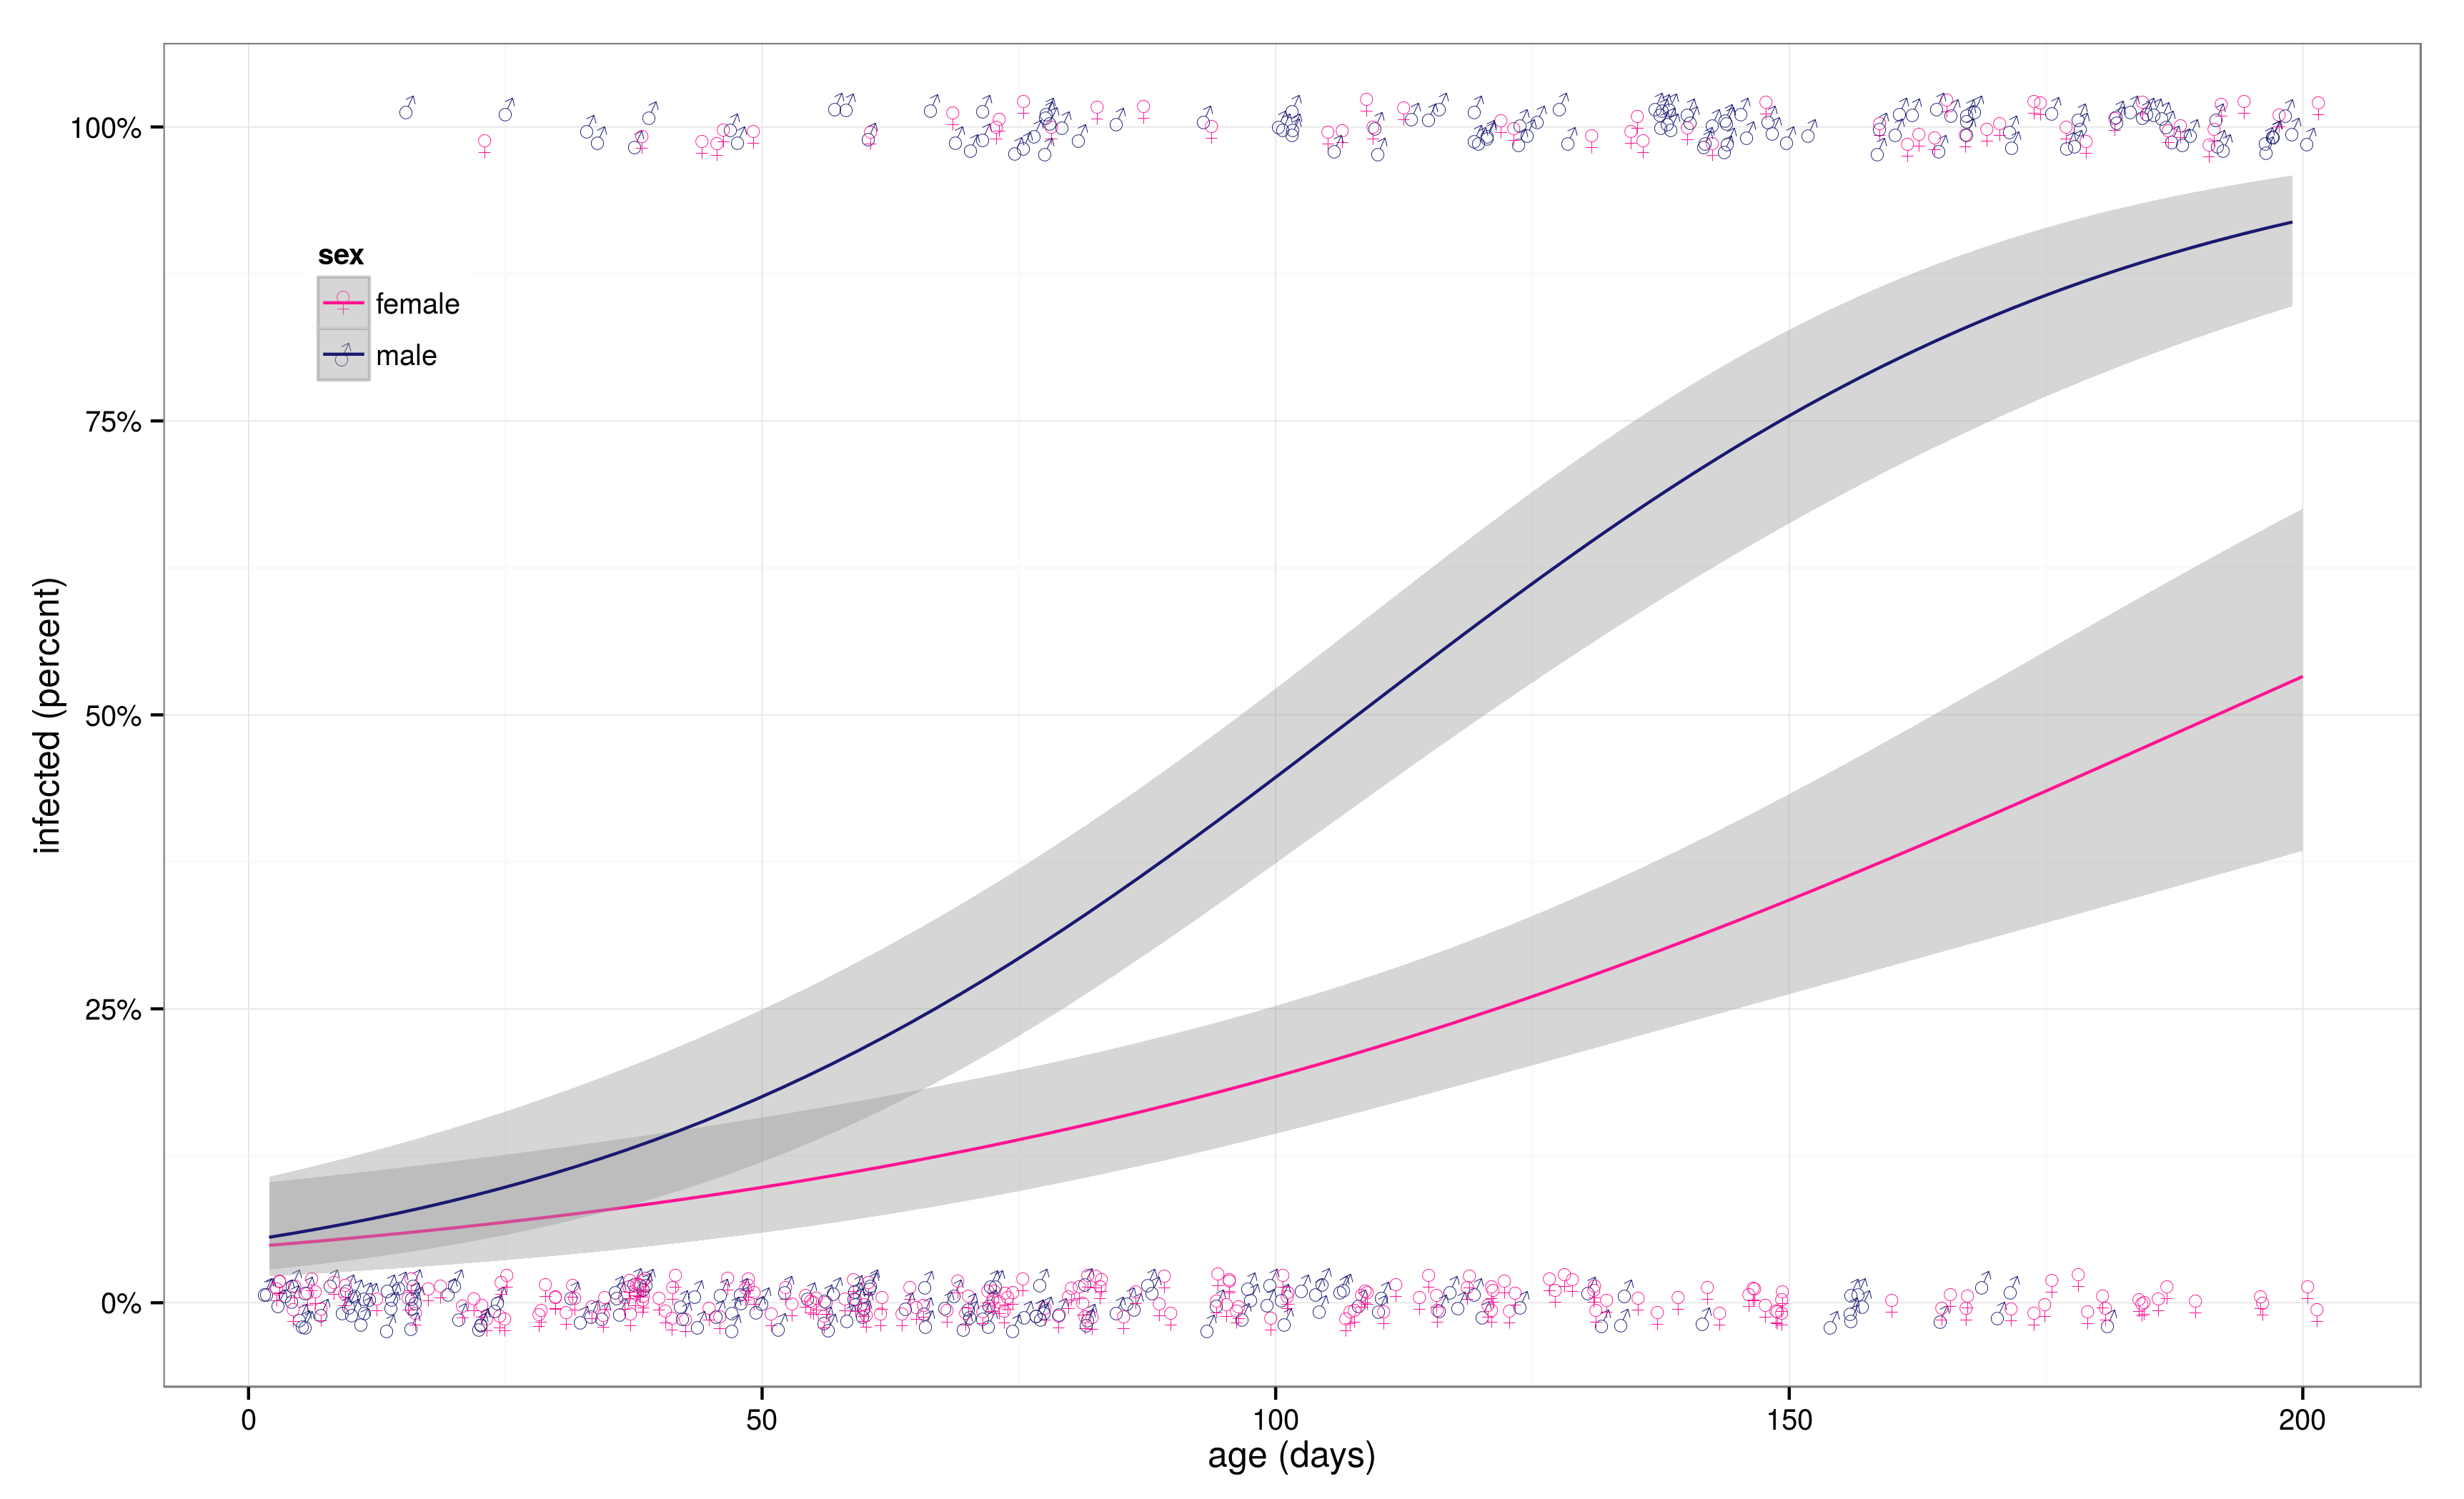
\includegraphics[width=11.5cm]{binancova1.png}
\end{center}
\end{frame}


\begin{frame}[fragile]\frametitle{Exercise}
Try to reproduce the plot! Hints:
  \begin{enumerate}
  \item set up a ggplot object, think about the aesthetics (\texttt{aes()}). Which quality of the graph you wanna set to which variable?
  \item begin with the lines (\texttt{geom\_smooth()})
  \item add the points (\texttt{geom\_jitter()}; do not think about the symbols in the first place; try to adjust the width and height appropriately)
  \item change the colour of the lines and points (\texttt{scale\_colour\_manual()}); I used midnightblue for male and deeppink for female
  \item change the symbols (\texttt{scale\_shape\_manual()}); use
\begin{verbatim}
    values = c("male" = "\u2642","female" = "\u2640"))
\end{verbatim}
     as values
  \item set the axes titles
  \item change to text of the y axis to percentage
  \item etc
  \end{enumerate}
\end{frame}


